\appendix

\chapter{相机投影细节}

本文在相机标定和后续所有运算中均使用了OpenCV中默认的针孔相机和畸变模型。
为了完整性,这里形式化地描述了该相机投影模型$\pi(\delta_i, \cdot)$。

在该模型下,对于任意在世界坐标系下的点$\mathbf{X}\in \mathbb{R}^3$,其在第$i$个相机的成像平面的投影点$\mathbf{x}^{(i)}$可以通过如下方式计算(简洁起见,此后省略上标$(i)$):
首先,应用罗德里格斯公式\cite{rodrigues},将$\mathbf{X}$从世界坐标系转换到第$i$个相机的坐标系,即
\begin{align}
    \theta &= \left\|r\right\|_2 \\
    \hat{\mathbf{r}} &= \mathbf{r}/ \theta \\
    \mathbf{R} &= \cos(\theta) I + (1- \cos{\theta} ) \hat{\mathbf{r}} \hat{\mathbf{r}}^\mathsf{T} + \sin(\theta) \begin{bmatrix}
         0   & -\hat{\mathbf{r}}_z & \hat{\mathbf{r}}_y \\
         \hat{\mathbf{r}}_z & 0    & -\hat{\mathbf{r}}_x \\
        -\hat{\mathbf{r}}_y &  \hat{\mathbf{r}}_x & 0
    \end{bmatrix}\label{eq:rodrigues} \\
    \mathbf{X}' &= \mathbf{R} \mathbf{X} + \mathbf{t}\text{,}
\end{align}
然后,将$\mathbf{X}'$投影到第$i$个相机的成像平面,即
\begin{equation}
    \mathbf{x}'' = \begin{bmatrix}
        \mathbf{X}'_x / \mathbf{X}'_z \\
        \mathbf{X}'_y / \mathbf{X}'_z
    \end{bmatrix}\text{,}
\end{equation}
对$\mathbf{x}''$应用镜头畸变,即
\begin{equation}
    \mathbf{x}' = \left(1 + k_1 r^2 + k_2 r^4 + k_3 r^6\right) \mathbf{x}'' + \begin{bmatrix}
        2 p_1 \mathbf{x}''_x \mathbf{x}''_y + p_2 \left(r^2 + 2 (\mathbf{x}''_x)^2\right) \\
        p_1 \left(r^2 + 2 (\mathbf{x}''_y)^2\right) + 2 p_2 \mathbf{x}''_x \mathbf{x}''_y
    \end{bmatrix}\text{,}
\end{equation}
其中$r = \left\|\mathbf{x}''\right\|_2$。最后,将$\mathbf{x}'$映射到以左上角为原点的像素坐标系,即
\begin{equation}
    \mathbf{x} = \begin{bmatrix}f_x & 0 \\ 0 & f_y \end{bmatrix} \mathbf{x}' + \begin{bmatrix}c_x \\ c_y \end{bmatrix}\text{。}
\end{equation}

\chapter{被动同步控制器实现细节}

\begin{figure}
    \begin{minipage}{0.52\textwidth}
        \centering
        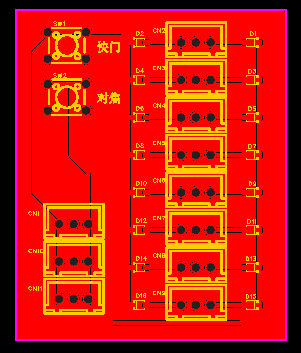
\includegraphics{figures/passive_sync_pcb}
        \captionof{figure}[被动控制器的PCB布局]{被动控制器的PCB布局。1:1尺寸比例}
        \label{fig:passive_sync_pcb}
    \end{minipage}\hfill%
    \begin{minipage}{0.45\textwidth}
        \centering
        \includegraphics{figures/2.5mm}
        \caption{用于焊接的2.5mm插头}
        \label{fig:2.5mm}
    \end{minipage}
\end{figure}
用于快门线接口的2.5mm插头如图\ref{fig:2.5mm}所示。
该插头的接触部分呈旋转对称的柱体,柱体不同高度上分布有3个独立的接触区域,分别对应对焦控制、快门控制和地线,
在插入相机时将会与相机内部电路连接。
其中两根控制线在相机待机时为带有上拉的输入端口,电压为3.3v。当其与地线短接,从而拉至低电平时,即可触发对应的控制。
此外,当手动按下相机快门按钮时,这些控制线也会输出低电平,以便于控制其他外设。

\begin{figure}
    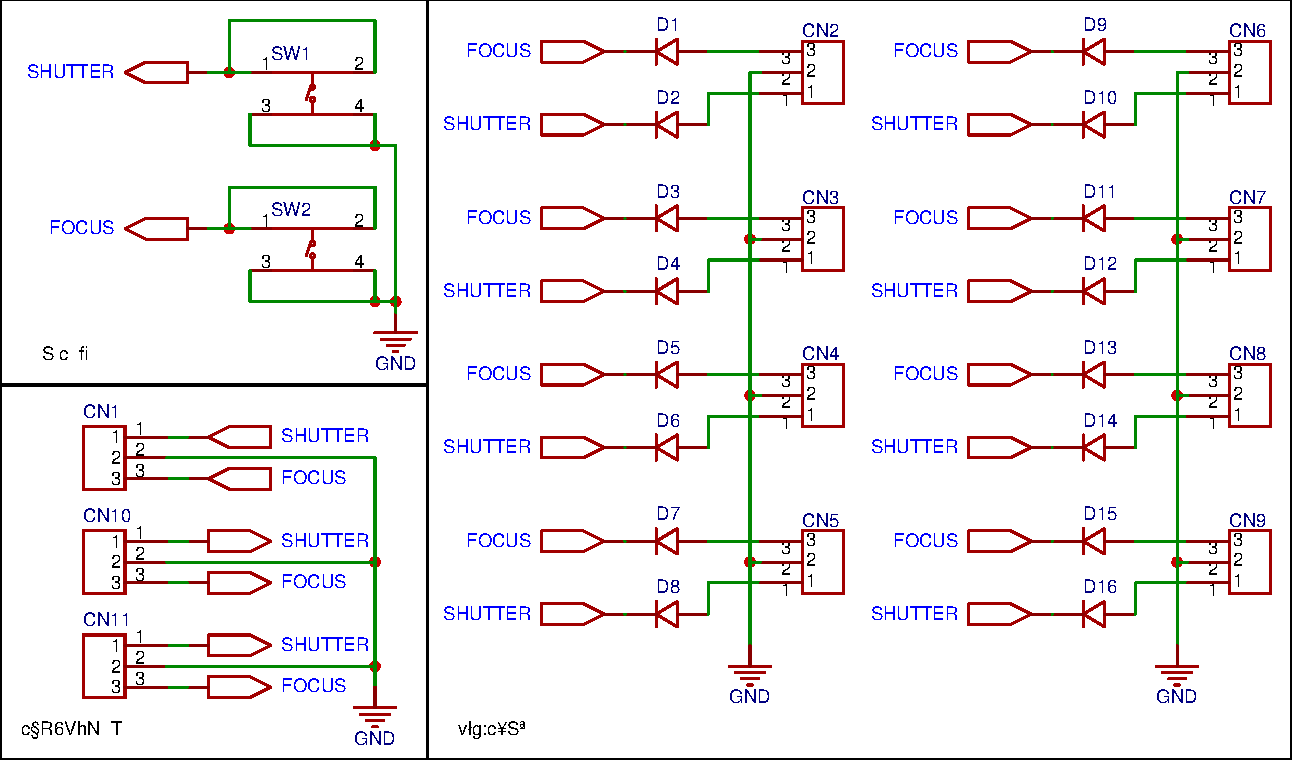
\includegraphics[width=\textwidth]{figures/passive_sync_schematic}
    \caption{被动控制器的电路原理图}
    \label{fig:passive_sync_schematic}
\end{figure}
每个被动控制器的电路原理图如图\ref{fig:passive_sync_schematic}所示,
该电路实现为一块简单的单面布线板,其布局如图\ref{fig:passive_sync_pcb}所示。
右侧8个XH2.54-3P插座用于连接相机,它们分别经过1N4148WS二极管后连接到合并的控制线上。
左侧3个XH2.54-3P插座则用于控制器之间的连接,不经过二极管。
左上角两颗$6\times 6$mm的轻触开关用于实现控制线与地线的短接,以便于触发对应的控制功能。


\chapter{主动同步控制器实现细节}

\begin{figure}[p]
    \centering
    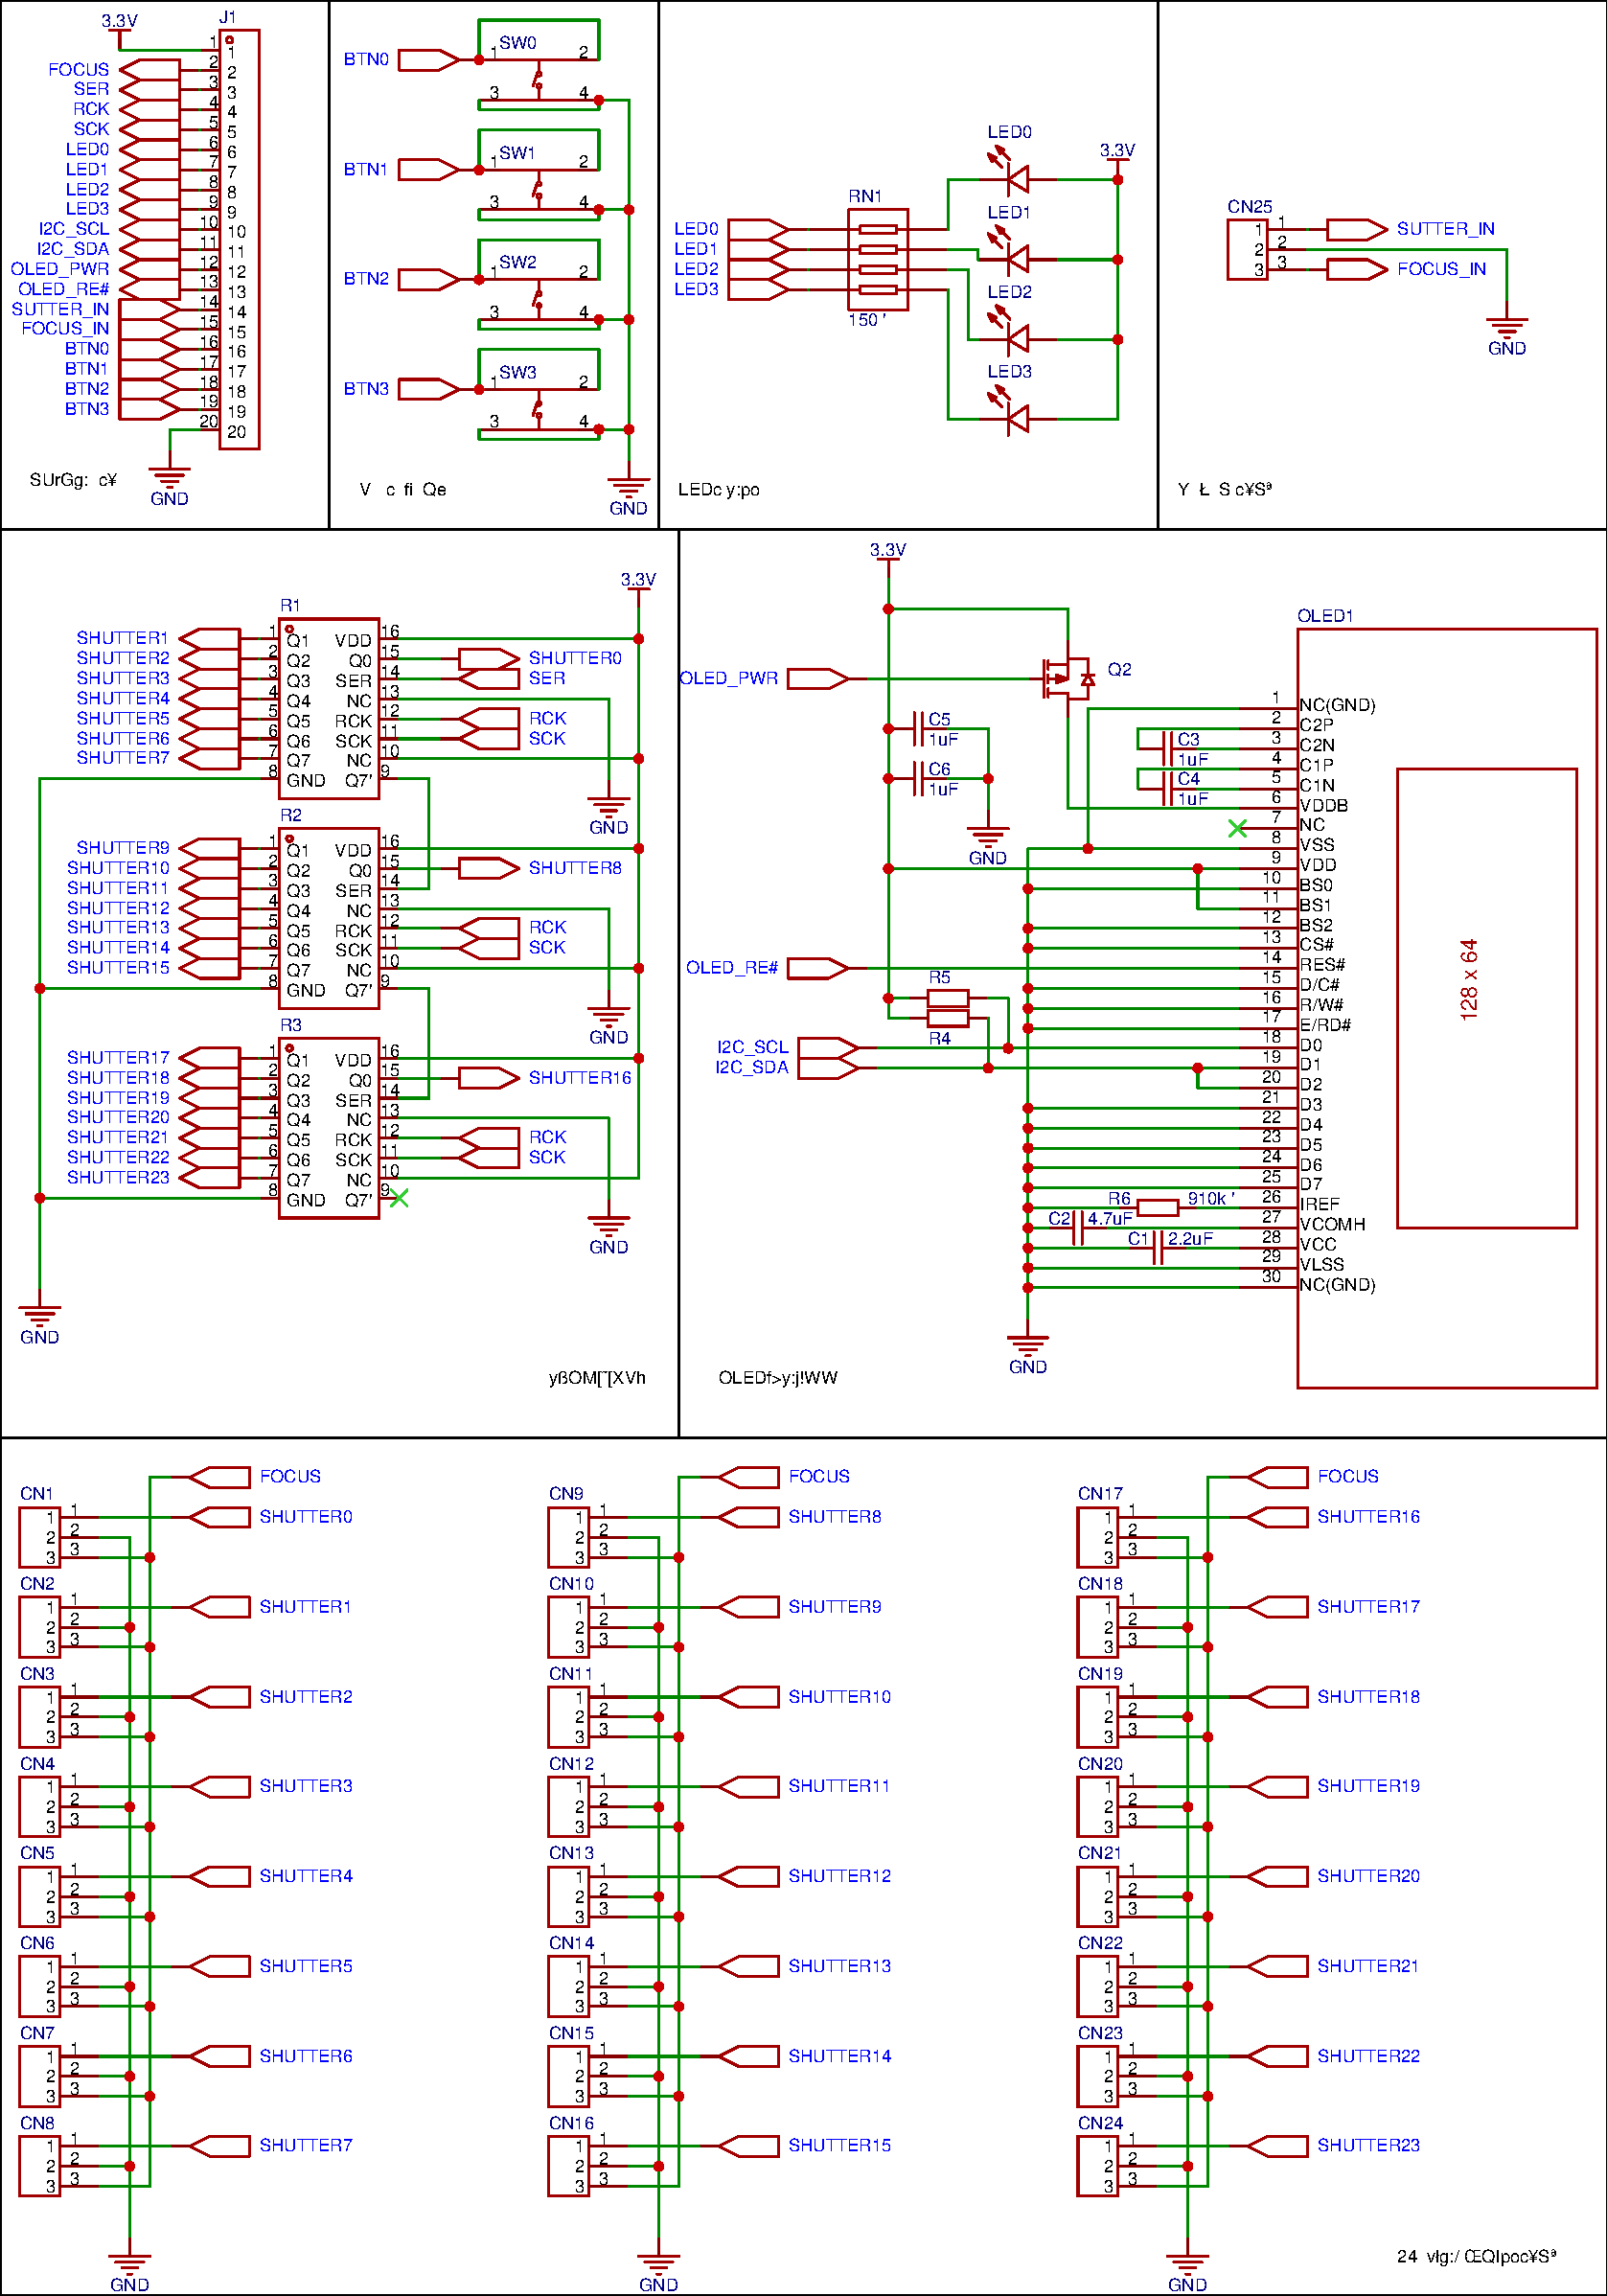
\includegraphics[width=\textwidth]{figures/active_sync_schematic}
    \caption{主动控制器的电路原理图}
    \label{fig:active_sync_schematic}
\end{figure}
\begin{figure}
    \centering
    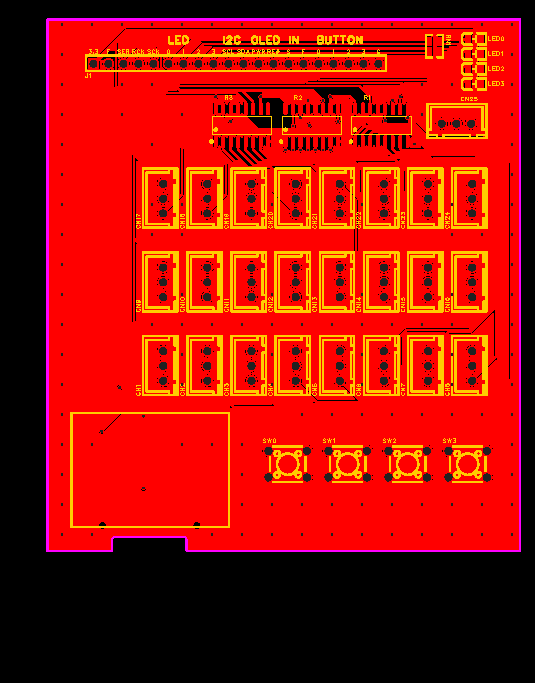
\includegraphics[page=1]{figures/active_sync_pcb}
    \includegraphics[page=2]{figures/active_sync_pcb}
    \caption[主动控制器的PCB布局]{主动控制器的PCB布局。1:1尺寸比例}
    \label{fig:active_sync_pcb}
\end{figure}
\paragraph{硬件}
主动同步装置的控制器实现为三块相互独立的电路板,
电路板之间使用20P的排针和排母连接。
其中包括一块市面上购买的STM32最小系统板,一块定制的布置了所有所需IO外设的IO板,
以及一块定制的用于连接两者的连接板。
之所以设计独立的一块连接版,是为了在不重新制作现有IO板的情况下,更改其与单片机的连接方式,也便于今后在同一片最小系统板上连接更多外设。
其中IO板的电路原理图如图\ref{fig:active_sync_schematic}所示。
该电路实现为一块双面布线的PCB,其布局如图\ref{fig:active_sync_pcb}所示。

其中OLED显示器使用SSD1306芯片,分辨率为$128\times 64$,显示区域尺寸0.96英寸。
STM32单片机通过硬件I2C接口与OLED显示器通信。
所采用的移位寄存器芯片为富满FM的74HC595D,其输出引脚的驱动方式为开漏输出,这可以避免不同独立供电的设备间电压不匹配造成的潜在问题。
在该方案中,每个相机的接口不再需要二极管,而可以直接连接到移位寄存器的输出引脚上。
其接口依然使用的是和被动同步控制器相同的XH2.54-3P插座,因此与相机和连接线可以共用。
OLED显示模块的电路设计则直接参考了相关数据手册中的参考电路。
但由于本方案中VDDB和VDD的供电来自同一条线路,因此省略了一个场效应管。

\clearpage
\paragraph{软件}
\begin{figure}
\centering
\begin{tikzpicture}[
    node distance=.2cm,
    every node/.style={outer sep=0pt,draw,anchor=south west},
    every fit/.style={inner sep=0pt},
    placeholder/.style={draw=none},
    fill_text/.style={draw=none,anchor=center},
    ]
    \node (event_p) [placeholder] {\vphantom{事件循环}};
    \node (btn) [above=of event_p.north west,anchor=south west] {按键检测};
    \node (ui_mgr_p) [placeholder,right=of btn] {\vphantom{图形界面管理}};
    \node (menu) [above=of ui_mgr_p.north west,anchor=south west] {菜单};
    \node (delay_overview) [right=of menu] {延迟概览};
    \node (num) [right=of delay_overview] {数值设置};
    \node (trigger) [right=of num] {触发};
    \node (about) [right=of trigger] {关于};
    \node (toast) [right=of about] {消息框};


    \node (oled_p) [above=of menu.north west,anchor=south west,placeholder] {\vphantom{OLED显示控制}};

    \node (oled_fit) [fit=(oled_p)(oled_p-|toast.east)] {};
    \node [fill_text] at (oled_fit) {OLED显示控制};

    \node (ui_mgr_fit) [fit=(ui_mgr_p)(ui_mgr_p-|toast.east)] {};
    \node [fill_text] at (ui_mgr_fit) {图形界面管理};

    \node (event_fit) [fit=(event_p)(event_p-|toast.east)] {};
    \node [fill_text] at (event_fit) {事件循环};

    \draw [->] (btn)++(0,2cm) -- node [left,draw=none] {中断} (btn);
\end{tikzpicture}
\caption{主动同步控制器的软件架构}
\label{fig:active_sync_software_arch}
\end{figure}
在主动同步控制器的单片机中运行的固件架构如图\ref{fig:active_sync_software_arch}所示。
该程序使用C++编写,不运行于操作系统之上。
该程序最外层为事件循环,它负责获取按键输入,将输入事件传递给图形界面模块,
并适时地休眠以节省电量。
按键检测模块负责响应按钮产生的硬件中断,产生输入事件,并过滤由于机械抖动产生的干扰信号。
图形界面管理模块负责维护当前打开的图形界面栈,处理打开新页面,和返回上一页面的请求,并将输入事件传递给栈顶的图形界面。
运行在图形界面管理模块之上的是各种具体的界面,它们负责真正处理输入事件,执行相应逻辑,并调用OLED显示控制模块来更新显示内容。
其中,菜单模块在构造时接收一个带有回调函数的菜单项列表,用于支持各种不同的菜单;
数值设置模块则使用traits模式,通过模板参数以支持不同的数值类型、数值范围和数值存储位置等,可支持触发延迟、休眠时间、屏幕对比度等诸多数值设置需求。
OLED显示控制模块负责调用单片机的硬件I2C接口与OLED显示器通信,
并封装了一些常用的绘图函数,如文本渲染等。

在菜单的导航中,从左到右四个按钮的功能分别定义为:上一项,确认,下一项,返回;
在数值设置界面,这些按钮则分别为:减小,切换开启/关闭,增大,确认。

值得一提的是,在延迟设置的界面,用户可设置的最小分辨率为0.1毫秒,且最大范围为5秒,共50000个不同的设置值。
但本装置只有4个按钮,为了能快速设置到需要的值,本文设计了一种特殊的交互方式。
当用户按住增大按钮时,数值将不断增大,其增大的速度分为三个阶段:
在按钮按下时数值增大0.1毫秒,0.5秒内不再增大;
在0.5秒到2秒内,数值每0.1秒增大0.1毫秒;
在2秒后,数值与按住的时间呈二次函数关系:若当前按钮按住的时间为$2+t$秒,最大设定值为$m=5$秒,设定数值的增量在之前线性增加的基础上,再额外增加$m(t/10)^2$,
即在10秒内数值增量相当于整个设置范围。
如此即可兼顾定位的准确性和大范围移动的便利性。
得益于本方案使用的traits设计模型,其他数值设置也能复用这一交互方式,只需在traits中定义好数值的范围,增量大小等即可。
在未来也可借助滚动编码器等额外硬件以提供更好的用户体验。
